% !TeX TS-program = pdflatex
\documentclass[xcolor={svgnames,x11names},
%draft
]{beamer}

\usepackage{tikzlings}
\usepackage{tikzducks}
\usetikzlibrary{positioning,shapes}

\setbeamertemplate{navigation symbols}{}
\setbeamertemplate{background canvas}{%
\begin{tikzpicture}[overlay, remember picture]
	\node[yshift=1.6cm] at (current page.center){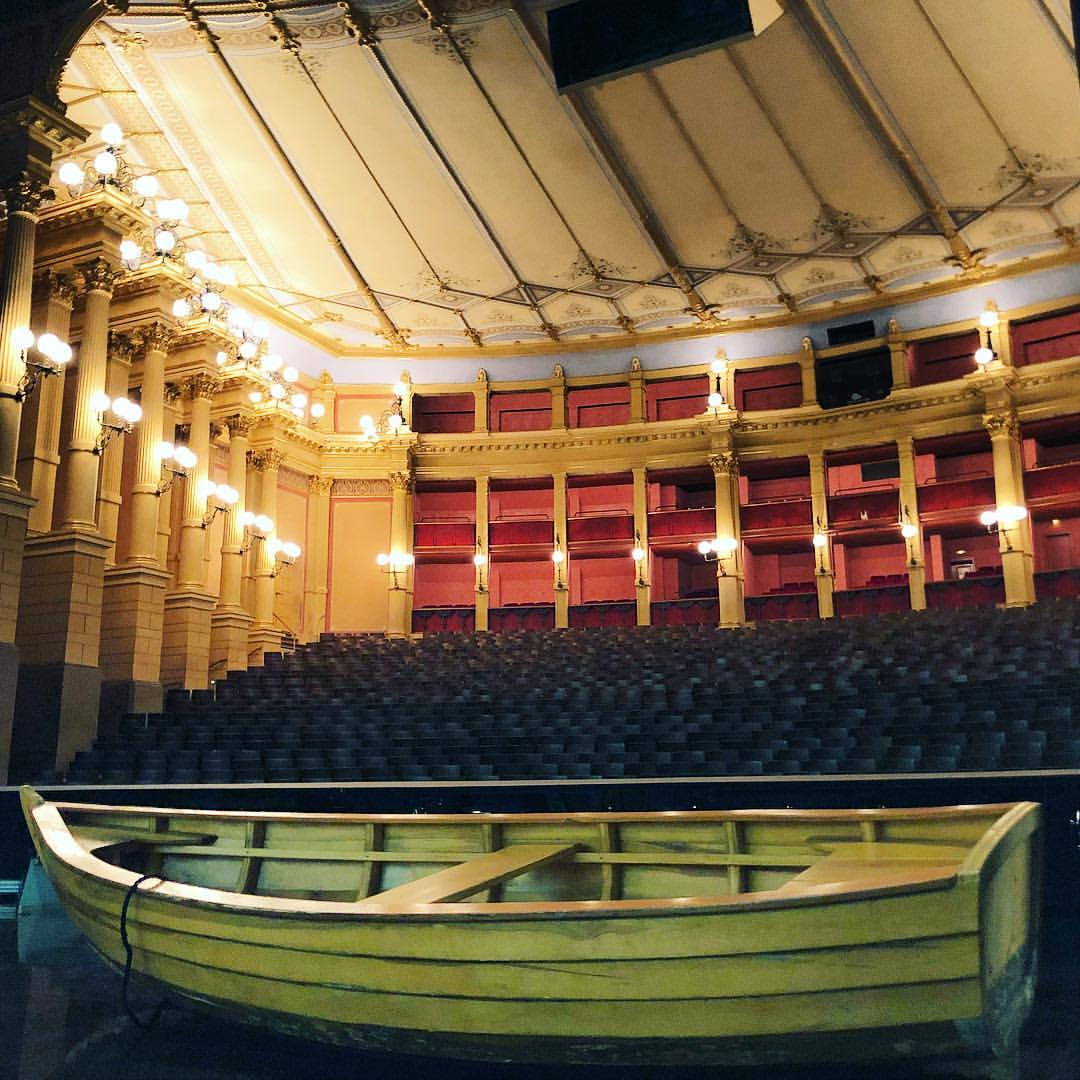
\includegraphics[width=\paperwidth]{Bayreuth}};
	\node[at=(current page.south),text width=.97\paperwidth,yshift=0.4cm,font=\tiny]{%
		\color{white}Backgrund image: \url{https://www.instagram.com/p/BmyRNlaFIv3/}\\
		Audio: \url{https://commons.wikimedia.org/wiki/File:Sound_Effects_-_Applause_after_a_concert.ogg}
};
\end{tikzpicture}
}

\begin{document}

\begin{frame}
\begin{tikzpicture}[remember picture, overlay]

% reihe 7
\node[
	xshift=7.4cm,
	yshift=-0.2cm+sin(10*\thepage)*cos(10*\thepage)*0.01cm
] at (0,0) {
	
\includegraphics[width=8.6cm,page=20]{rows}
};
\node[
	xshift=7.63cm,
	yshift=-0.2cm
] at (0,0) {
	
\includegraphics[width=8.6cm,page=19]{rows}
};
\node[
	xshift=7.87cm,
	yshift=-0.24cm+sin(10*\thepage)*sin(10*\thepage)*0.03cm
] at (0,0) {
	
\includegraphics[width=8.6cm,page=18]{rows}
};
\node[
	xshift=8.1cm,
	yshift=-0.22cm
] at (0,0) {
	
\includegraphics[width=8.6cm,page=17]{rows}
};

% reihe 4
\node[
	xshift=6.8cm,
	yshift=-0.5cm+sin(10*\thepage)*cos(10*\thepage)*0.04cm
] at (0,0) {
	
\includegraphics[width=9.3cm,page=16]{rows}
};
\node[
	xshift=7.03cm,
	yshift=-0.53cm
] at (0,0) {
	
\includegraphics[width=9.3cm,page=15]{rows}
};
\node[
	xshift=7.27cm,
	yshift=-0.54cm+sin(10*\thepage)*sin(10*\thepage)*0.03cm
] at (0,0) {
	
\includegraphics[width=9.3cm,page=14]{rows}
};
\node[
	xshift=7.5cm,
	yshift=-0.5cm
] at (0,0) {
	
\includegraphics[width=9.3cm,page=13]{rows}
};


% reihe 3
\node[
	xshift=6.2cm,
	yshift=-0.9cm+sin(10*\thepage)*cos(10*\thepage)*0.06cm
] at (0,0) {
	
\includegraphics[width=10cm,page=12]{rows}
};
\node[
	xshift=6.47cm,
	yshift=-0.91cm
] at (0,0) {
	
\includegraphics[width=10cm,page=11]{rows}
};
\node[
	xshift=6.73cm,
	yshift=-0.93cm+sin(10*\thepage)*sin(10*\thepage)*0.07cm
] at (0,0) {
	
\includegraphics[width=10cm,page=10]{rows}
};
\node[
	xshift=7cm,
	yshift=-0.9cm
] at (0,0) {
	
\includegraphics[width=10cm,page=9]{rows}
};

% reihe 2
\node[
	xshift=6cm,
	yshift=-1.3cm+sin(10*\thepage)*cos(10*\thepage)*0.08cm
] at (0,0) {
	
\includegraphics[width=10.5cm,page=8]{rows}
};
\node[
	xshift=6.25cm,
	yshift=-1.34cm
] at (0,0) {
	
\includegraphics[width=10.5cm,page=7]{rows}
};
\node[
	xshift=6.5cm,
	yshift=-1.32cm+sin(10*\thepage)*sin(10*\thepage)*0.06cm
] at (0,0) {
	
\includegraphics[width=10.5cm,page=6]{rows}
};
\node[
	xshift=6.75cm,
	yshift=-1.3cm
] at (0,0) {
	
\includegraphics[width=10.5cm,page=5]{rows}
};

% reihe 1
\node[
	xshift=6cm,
	yshift=-1.7cm+sin(10*\thepage)*cos(10*\thepage)*0.07cm
] at (0,0) {
	
\includegraphics[width=11cm,page=4]{rows}
};
\node[
	xshift=5.75cm,
	yshift=-1.74cm
] at (0,0) {
	
\includegraphics[width=11cm,page=3]{rows}
};
\node[
	xshift=5.5cm,
	yshift=-1.7cm+sin(10*\thepage)*sin(10*\thepage)*0.10cm
] at (0,0) {
	
\includegraphics[width=11cm,page=2]{rows}
};
\node[
	xshift=6.25cm,
	yshift=-1.72cm
] at (0,0) {
	
\includegraphics[width=11cm,page=1]{rows}
};

\node at (9.7,-2.2) {
\includegraphics[width=1.5cm]{viking_back}};
\node[xscale=-1] at (4.5,-2.4) {
\includegraphics[width=1.5cm]{viking_back}};

\end{tikzpicture}
\pause[100]
\end{frame}

%\setbeamercolor{background canvas}{bg=}
%\foreach \x in {1,...,100}{
%	\includepdf{cheering-credits.pdf}
%}

\end{document}
